\documentclass[b5paper]{article}
%\usepackage[utf8]{inputenc}

%\usepackage{fontspec}
%\setmainfont{Linux Libertine O}

\usepackage{polyglossia}
\usepackage{amsmath}
\usepackage{multirow}
\usepackage{amsfonts}
\usepackage{amssymb}
\usepackage{breqn}
\usepackage[parfill]{parskip}
\usepackage{tikz}
\usepackage{float}
\usepackage{epstopdf}
\usepackage{color}
\usepackage{fontspec}
\usepackage{xunicode}
\usepackage{xltxtra}
\usepackage{fancyhdr}
\usepackage{expex}
\usepackage{bm}

\usepackage{tablefootnote}


\usepackage{url}

\usepackage{subcaption}

\usepackage[left=1.65cm,right=1.65cm,top=2cm,bottom=2cm]{geometry}
%\chead{\textsc{\small }}
%\rhead{}
%\lfoot{}
%\cfoot{\thepage}
%\rfoot{}
%\pagestyle{fancy}

\makeatletter
\def\blfootnote{\gdef\@thefnmark{}\@footnotetext}
\makeatother

\setmainfont[Mapping=tex-text]{Linux Libertine O}

\newcommand{\todo}[2]{{\textcolor{red}{\bf [#1] #2 }}}
\newcommand{\note}[1]{{\textcolor{blue}{#1}}}

\newcommand{\ns}{Northern Sámi}
\newcommand{\ngram}{$n$-gram}

\newcommand{\ds}[1]{\textsc{#1}}

\title{Automatic Speech Recognition for \ns\ with comparison to other Uralic Languages\blfootnote{
    This work is licensed under a Creative Commons Attribution–NoDerivatives
    4.0 International Licence.  Licence details:
    \url{http://creativecommons.org/licenses/by-nd/4.0/}
}} 
\author{
\makebox[.45\linewidth]{Peter Smit\textsuperscript{1}}\\
\texttt{peter.smit@aalto.fi}
\\
\and 
\makebox[.45\linewidth]{Juho Leinonen\textsuperscript{1}}\\
\texttt{juho.leinonen@aalto.fi}
\\
\and 
\makebox[.45\linewidth]{Kristiina Jokinen\textsuperscript{2}}\\
\texttt{kristiina.jokinen@helsinki.fi}
\and
\makebox[.45\linewidth]{Mikko Kurimo\textsuperscript{1}}\\ 
\texttt{mikko.kurimo@aalto.fi}
\\ 
\and
\small\textsuperscript{1}Department of Signal Processing and Acoustics, Aalto University, Finland \\
\small\textsuperscript{2}Institute of Behavioural Sciences, University of Helsinki, Finland\\
}


\begin{document}

\maketitle

\begin{abstract} 
Speech technology applications for major languages are becoming widely available, but for many other languages there is no commercial interest in developing speech technology. As the lack of technology and applications will threaten the existence of these languages, it is important to study how to create speech recognizers with minimal effort and low resources.

As a test case, we have developed a Large Vocabulary Continuous Speech Recognizer for \ns, an Finno-Ugric language that has little resources for speech technology available. Using only limited audio data, 2.5 hours, and the \ns\ Wikipedia for the language model we achieved 7.6\% Letter Error Rate (LER). With a language model based on a higher quality language corpus we achieved 4.2\% LER. To put this in perspective we also trained systems in other, better-resourced, Finno-Ugric languages (Finnish and Estonian) with the same amount of data and compared those to state-of-the art systems in those languages. 
\end{abstract}

\section{Introduction}

The field of speech recognition is maturing, as companies start to actively use and sell products that utilize Large Vocabulary Continuous Speech Recognition (LVSCR). Especially the creators of operating systems for mobile devices incorporate methods into their products to operate devices using voice.

These commercial applications however, are only focusing on small fraction of the languages in the world. Other languages do not have the required data and expertise readily available, and are therefore left out from these systems as it would not be commercially viable to create these applications. Especially minority languages and languages from developing countries receive only minor academic and commercial interest for the development of LVCSR systems. \cite{besacier2014automatic}

One for these under-resourced languages is \ns, the largest of the nine Sámi languages with approximately 25,000 speakers. It belongs to the Uralic language family. \cite{ethno18}

Like other languages in the Finno-Ugric branch of the Uralic language family, e.g. Finnish and Estonian, it is a highly morphological language that uses independent suffixes extensively. This poses challenges for speech technology applications as the number of inflections, derivations and compoundings cause the size of the vocabulary to be enormous, especially compared to the languages in the Indo-European family \cite{karlsson1982}.  A large vocabulary especially causes problems in the estimation of language models, which can not produce any words beyond those seen in the the training data. 

\ns\ is an under-resourced language, as there are little corpora of spoken and written language available, and financial resources to collect these data are limited. Even though there is active linguistic research on \ns, there are limitations to the expert resources available for speech recognition, such as pronunciation dictionaries. 

To combat the challenges of building an LVCSR system for an under-resourced language we have employed several techniques. First we used `found data' for building the acoustic and language models. For the acoustic model we bootstrapped from a better resourced related language (Finnish). For the language model we increased the coverage of the model by employing sub-word units (morphs) instead of words. Similar techniques have been used in \cite{besacier2014automatic,viet2009} but here we wanted to evaluate their applicability to uralic languages, in particular. This work is an extension of \cite{leinonen2015}.

%To project a possible upper-bound on the recognition accuracies possible for \ns, we also have produced systems for Finnish and Estonian, using the same quantities of data for comparison. Comparing these to the state-of-the art systems for Finnish and Estonian will give a good estimate of the possible gains before more \ns\ data is gathered.

Because there are no state-of-the-art LVCSR references for \ns, we simulated the potential of larger resources by studying also two better resourced Uralic languages. First we produced systems for Finnish and Estonian using the corresponding data as we had for \ns. Then we compared these systems to similar systems that we produced using larger data and, finally, to the state-of-the art systems for these languages. These results helped us to estimate the gains for collecting more \ns\ data.


\subsection{WikiTalk and DigiSami}
Another motivation to build a recognizer for \ns\ is to utilize it as part of  a spoken dialogue system in the WikiTalk application \cite{wilcock2013wikitalk}. This is one part of the DigiSami project which is a research project at University of Helsinki aiming to support content generation of less resourced languages with the help of language technology. Currently, the main dangers to Sámi language are the disappearance of the traditional lifestyle and work of Sámi culture, and emigration of Sámi people away from their old living areas. However, there are also studies and discussion on using new technologies to revitalize languages \cite{eisenlohr2004language}. In \cite{jokinen2014open}, revitalization for the \ns\ language is described using spoken language data collection in interactive setting for the WikiTalk application. In WikiTalk, the idea is to have users (children or adults) find out more about subjects that interest them by discussing with the humanoid robot Nao. They can ask for more information on the subject and then Nao will read them the related Wikipedia article \cite{jokinen2014multimodal}. Described in this paper is the first step to building this end-to-end system.


\section{ASR for under-resourced languages}
The majority of the state-of-the art methods in Large Vocabulary Speech Recognition require large amounts of data and expertise. 

Firstly, a great number of high quality spoken utterances have to be collected and correctly transcribed. For a Speaker-Independent (SI) system, i.e. a system that can recognize anyone who speaks the target language, utterances from many different persons are needed. For a Speaker-Dependent (SD) system, i.e. a system that can only recognize the voice of the person who provided the training data, only a few hours of transcribed speech are required.

The second required dataset is a large corpus of written text, preferably in the same style and domain as what should be recognized by the system. Te corpus is used to train the language model and it should contain all common words in their expected contexts.

Lastly, a speech recognizer needs a pronunciation dictionary; i.e. a list of all possible words with all their possible phonetic transcriptions. The phonemes also need to be grouped according to different phonetic properties, so that their probability distributions can be shared in the training of the acoustic model.

For under-resourced languages, as the name suggests, none of the above data is readily available, but alternative solutions have to be developed. An easy alternative to a large corpus of transcribed audio data is to collect audio books. Although the quality of the speech varies, projects such as Librivox have freely available audio books in many languages which can be used for this purpose. Using a temporary acoustic model and simple text processing techniques these audio books can be automatically segmented into sentence-long utterances that are suitable for training a minimal speaker-dependent model.

Language data is also freely available on-line, and e.g. Web-scraping can give a rudimentary dataset for training a language model \cite{scannell2007crubadan}.  Also sites like Wikipedia have often big collections of easily available text. However, the quality and usability of such data varies, and many of the sources that can be `found' on-line suffer from the problem that their style and topic are non-standard and do not necessarily match written nor spoken language conventions. Moreover, on-line texts often contain foreign language segments, symbols or abbreviations which decrease their usability for building language models.

One of the main resource consuming tasks is the preparation of a pronunciation dictionary, which normally requires extensive manual work and linguistic knowledge. One solution to build the pronunciation dictionary quickly is to model the graphemes (letters) of the words directly, instead of using the actual phone they represent \cite{kanthak2003multilingual}. In languages such as English this does not, of course, give very good results since graphemes can have very different realizations. Consider for example the words `tough' and `dough' that resemble each other in writing, but are pronounced in a completely different way. In the Uralic languages studied here however, a grapheme-to-sound system works reasonably well since, in general, every grapheme is realized as a single distinct sound.

Lastly, the phonetic grouping or `phoneme question set' is a small dataset that requires linquistic expertise. Although there are algorithms available that can replace this set altogether \cite{darjaa2011effective}, it is often undesirable as it makes the system less effective. it is also possible to modify the phoneme set of a closely related language, and such small modifications to approximate the target language do not necessarily require so much expert effort.

Even though the above simplified solutions can replace all the expensive data needs, they will inevitably limit the performance of the speech recognizer. Adding more and domain related training data as well as developer expertise will naturally improve the system performance significantly. However, the low-resource systems can already serve some basic language technology needs. The largest limiting factor for these systems is that a real SI system requires training data from more than a hundred speakers.


\section{Acoustic modeling}
\label{sec:align}
The Acoustic Modeling part of the speech recognizer was done with a standard Hidden Markov model with Gaussian mixture models as emission distribution (HMM-GMM). Mel Frequency Cepstral Coefficients were used as input features. \cite{hirsimaki2009importance}

The audio data is prepared by splitting the audio files (originally chapter length or similar) into sentence utterances. This is done by doing Baum-Welch forced alignment with a temporary speech recognition model. The temporary speech recognition model was created by taking a well trained Finnish model and mapping the Finnish phonemes to the one of the target language. In later iterations the best speech recognition model of the language was used to do the forced alignment again, resulting in a perfect split of training utterances.

The HMM-GMM model is trained using multiple iterations of Baum-Welch maximum likelihood estimation. To manage the model complexity Gaussians were shared between different HMM-states using decision tree clustering. The modeling unit of the acoustic model is a tri-state tri-phone, which means that all the phonemes with a different preceding and succeeding phoneme are modeled as separate units, as are the beginning, middle and end of each tri-phone.

In Section~\ref{sec:compexp} the number of Gaussians for different models are reported.


\section{Language modeling}

A language model is an important part of any speech recognition system. Even though theoretically a good acoustic model with a lexicon could be enough to recognize words, a model that takes the word context is essential. For languages which have many homophones, i.e. words with the same pronunciation but different meaning, it is also essential to have a language model, so as to pick the right word meaning given a pronunciation in the context. 

%\ngram\ models predict the output of the next word given the $n-1$ previous words. 

A language model predicts words based on their sentence context. For synthetic languages like Finnish and all the Uralic languages, the main issue with word-based language modeling is that a huge lexicon is needed in order to decrease the out-of-vocabulary (OOV) rate to a manageable percentage. Since the OOV-rate is the minimum WER possible, an OOV-rate much less than 10\% is necessary. For an English speech recognizer, a vocabulary size of 20 000 word may provide an OOV-rate of 2.4-2.7\%, while with a vocabulary of 40 000 words, an OOV-rate less than one percent is achieved \cite{woodland19951994}. In contrast, a Finnish recognizer needs a 410 000 word vocabulary to have an OOV-rate of 4.0-7.3\% \cite{hirsimaki2006unlimited}.

An interesting alternative for a word-based language model is to use a sub-word language model. A sub-word model builds words out of a smaller set of word fragments. The word fragments are particularly effective in agglutinative languages or languages with a lot of compound words. When the words are built from smaller units, also the OOV words can be modelled by using the probabilities of sub-word unit combinations learned from the training corpus. If the word fragments are chosen correctly, the OOV-rate can become close to zero, even for smaller language data corpora.

\subsection{Morfessor}
Morfessor is a machine learning tool that uses a statistical model to split words into smaller fragments, which can be used for language modeling \cite{creutz2007unsupervised}. This resembles closely the splitting of words into their smallest informational units, morphemes. 

Morfessor has three components; the model, the cost function, and the training and decoding algorithms. The model contains the lexicon, i.e. the properties of the morphs, the written form of the morph itself and its frequency, as well as the grammar, which contains information of how the morphs can be combined into words. The Morfessor cost function is derived from a MAP estimation with the goal of finding the optimal parameters $\bm{\theta}$ given the observed training data $\bm{D}_W$:

\begin{equation}
\bm{\theta}_{MAP}=\operatorname*{arg\,max}_{\theta}P(\bm{\theta}|\bm{D}_W)=\operatorname*{arg\,max}_{\theta}P(\bm{\theta})P(\bm{D}_W|\bm{\theta}).
\end{equation}

The cost function to be minimized is the negative logarithm of the product  $P(\bm{\theta})P(\bm{D}_W|\bm{\theta})$

\begin{equation}
L(\bm{\theta}, \bm{D}_W)=-\log P(\bm{\theta})-\log P(\bm{D}_W|\bm{\theta}).
\end{equation}

The purpose of this is to generate a small set of morphs that represents the words in the training corpus compactly. If only letters were used as morphs the set of would be small but representing the corpus with individual letters would be cumbersome. In contrast using whole words as morphs would result in a large set of morphs so the optimal solution is somewhere in between. However, individual letters are added to the morph set so even previously unseen words can always be segmented.

A greedy search algorithm is used to find the optimal segmentation of morphs for the training data.  When the best model is found, it is used to segment the language model training corpus with the Viterbi algorithm. This result can be used to generate \ngram\ models with morphs as LM units.



\subsection{\ngram\ modeling}

\ngram\ models predict the output of the next word or sub-word given the $n-1$ previous words or sub-words. They are normally created by counting all occurrences of the word and sub-word sequences. To prevent the model from being too big and too much tailored to the training data (overfitting), pruning is applied. Also, some of the probability mass is reserved for unseen contexts, for example with the Kneser-Ney smoothing technique\cite{chen1996empirical}.

When \ngram\ models are build for words, the order the model, i.e the value of $n$, is typically between three and five. If the order is high, the models get too big, and they do not contain enough necessary information. With the sub-word models, however, the contexts can be much deeper, as there are less types in the vocabulary and the context counts are more sparse. Also intuitively, to cover the same context, the order of a sub-word model must be higher than the order or the word model.
Standard tools for \ngram\ modelling have problems with correctly smoothing and growing high-order \ngram\ language models.  VariKN  \cite{siivola2007growing} is a specific algorithm and tool to solve this problem and it was used in this paper for building high-order sub-word  \ngram\ models. 

%Also for For decoding we have used the AaltoASR decoder, which is specialized in decoding morph-language models with deep contexts.


\section{Experiment setup}

%\note{we don't have to explain acoustic modeling, language modelling etc. We do need to tell what recognizer we used (AaltoASR) and what features it has (MFCC's, Gaussian-mixture HMM's, type of decoder). Same for language modeling tools}


The experiments were carried out using our open source speech recognition toolkit called AaltoASR\footnote{Open source, available from \url{https://github.com/aalto-speech/AaltoASR}} \cite{hirsimaki2009importance}\cite{pylkkonen2005efficient}. It uses context-dependent tri-phones with diagonal Gaussian mixture models (GMM) as emission distributions and the speech features itself are Mel-Frequency Cepstral Coefficients (MFCCs). 

Both words and sub-word units were used for language modeling. The sub-word unit models were created with Morfessor 2.0\footnote{Open source, available from \url{http://www.cis.hut.fi/projects/morpho/}}, an implementation of the Morfessor Baseline algorithm\cite{virpioja2013morfessor}. 

Variable length \ngram s used for language modeling were generated by both SRILM\footnote{Open source, available from \url{http://www.speech.sri.com/projects/srilm/}} \cite{stolcke2002srilm} and VariKN\footnote{Open source, available from \url{https://github.com/vsiivola/variKN}} \cite{siivola2007growing,siivola2007morfessor}. The decoder of AaltoASR is a time-synchronous one-pass token passing decoder where the beam search is complemented by a language model look-ahead \cite{ortmanns1997look}.

%Important parameters of the models (the number of samples used to estimate a Gaussian, the $\alpha$-parameter of the Morfessor model, and the language model weight used during decoding), were evaluated during the experiment setup using a development set, but kept at their respective defaults as they did not give significant improvements.



\section{\ns\ ASR evaluation} 
\label{sec:samiexp}
The audio data used for the \ns\ recognizer came from the UIT-SME-TTS corpus\footnote{Provided by the University of Tromsø}. There are data for two speakers, one male and one female. The male audio data was 4.7 hours and the female data 3.3 hours. Separate data is needed for development and evaluation, and we used 75\% for training. This makes 3.5 and 2.5 hours for the male and female voice, respectively.

The initial recognition model was created by using a Finnish model. With this model, the audio data was split into sentences and trained with the procedure described in Section~\ref{sec:align}. This resulted in two speaker dependent systems, one for the male and one for the female speaker (resp. SM1 and SF1). These models are Speaker-Dependent models as there is data only from the two speakers available.

For language model, we evaluated both word and morph \ngram\ models. In addition to the training sentences, we also used the \ns\ Wikipedia dump (\ds{Train+Wiki}).

The results for basic recognition are shown in Table~\ref{tbl:samibasic}. Besides the standard Word Error Rate (WER), also the Letter Error Rate (LER) is reported. LER is common for speech recognition experiments on languages which are morphological complex such as \ns, Finnish and Estonian.

\begin{table}[!h]
\centering
\begin{tabular}{ll|rrr|rrr}
& & \multicolumn{3}{|c|}{\textbf{Speaker SF1}} & \multicolumn{3}{|c}{\textbf{Speaker SM1}} \\
 \textbf{Unit} & \textbf{Toolkit} & \textbf{5-gram} & \textbf{7-gram} & \textbf{9-gram} & \textbf{5-gram} & \textbf{7-gram} & \textbf{9-gram}\\\hline
 words & SRILM & 52.9 / 12.7 & 52.9 / 12.7& 52.9 / 12.7&48.6 / 11.1 & 48.7 / 11.1 & 48.7 / 11.1\\
morphs & SRILM & 40.0 /  9.0 & 39.9 / 9.3& 39.1 / 9.1 & 37.6 / 8.5 & 36.8 / 8.4 & 37.3 / 8.5 \\
 morphs & VariKN  & 38.4 / 8.6& 38.5 / 8.7  & 37.6 / 8.7 & 35.4 / 8.1 &  33.7 / 7.6 & 34.1 / 7.9 \\
%DST & words & SRILM & & & & & & \\
%DST & morphs & SRILM & & & & & & \\
%DST & morphs & VariKN  & & & & &  & \\ 

\end{tabular}
\caption{ASR recognition results for the \ns\ SD recognizers. Word Error Rate / Letter Error Rate reported.\label{tbl:samibasic}}
\end{table}


We first observe that the SM1 recognizer is slightly better than the SF1 recognizer. However, this is most likely caused by the fact that there was more data available for the training of the acoustic model.

As expected, the morph based language models have much lower error rates than the word-based models. Looking at Table~\ref{tbl:samioov}, we notice that the OOV-rate for word based models is rather high which causes the big difference in performance to sub-word models. %TODO

\begin{table}[!h]
\centering
\begin{tabular}{lrr}
& Word & Morph\\\hline
Female &  22\% & 0\% \\
Male & 20\% & 0\%\\
\end{tabular}
\caption{Out-of-vocubulary percentages for the Female and Male testsets. \label{tbl:samioov}}
\end{table}


For word-based models there is no effect on using higher order \ngram s. This can be seen in Figure~\ref{fig:samiperf}  which shows WER for different \ngram\ models with the SM1 system. In this comparsion we used the\ds{Big} \ns\ language model which is trained from approximately 12 million word tokens of data from `Den samiske textbanken'. There is no change in performance after the 3rd order \ngram s for the the word-based model, whereas for the VariKN morph-based models there are clear effects when using higher order models. To model the same context as a word model, more units of a sub-word model are needed. The SRILM tool does not do very well on this morph data, which is caused by the limited smoothing/growing algorithms of SRILM. %TODO unclear

The best Word Error Rate on the \ds{Big} language model for the SM1 system is 18.2\%, the best Letter Error Rate 4.2\%. 

\begin{figure}
\centering
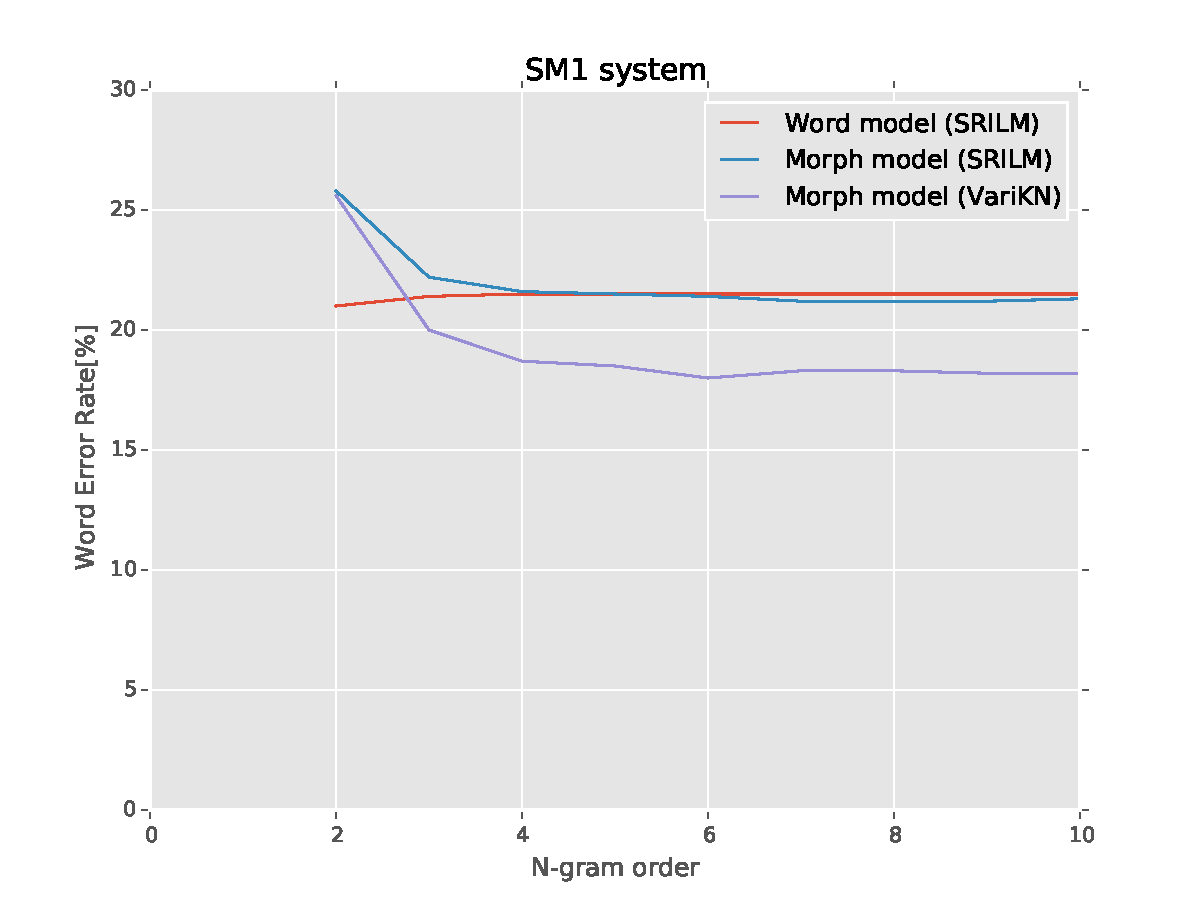
\includegraphics[width=.9\textwidth]{figures/sme1}
\caption{Word error rates for the SM1 system with the \ds{Big} language model.}\label{fig:samiperf}

\end{figure}



%The last observation is that the VariKN toolkit does a better job in creating a high-order ngram model for morph models. This is expected as it is specifically designed to be used for this purpose.


\section{Comparison of low-resource systems for multiple languages}
\label{sec:compexp}
To compare the results of the \ns\ recognizer with recognizers in different languages we first train Speaker Dependent models for both Finnish and Estonian audio books. The available audio datasets are described in Table~\ref{tbl:amdatacomp} and the available text corpora in Table~\ref{tbl:lmdatacomp}. 


\begin{table}
\centering
\begin{tabular}{llllr}
 & \textbf{Language} & \textbf{Gender} & \textbf{Title} & \textbf{Amount}\\\hline
EF1 & Estonian & Female &Nils Holgerssoni imeline teekond läbi Rootsi  & 16 hours \\
EM1 & Estonian & Male & Würst Gabriel ehk Pirita kloostri wiimsed päewad & 6 hours \\
FF1 & Finnish & Female & Syntymättömien sukupolvien Eurooppa & 12 hours\\
FM1 & Finnish & Male & Seitsemän veljestä\tablefootnote{Provided by YLE. Can be listened on  \url{http://areena.yle.fi/1-1301621}} & 13 hours\\
SF1 & \ns & Female & UIT-SME-TTSF & 3.3 hours  \\
SM1 & \ns & Male & UIT-SME-TTSM & 4.6 hours \\
\end{tabular}
\caption{Audio data for the trained speaker dependent systems.\label{tbl:amdatacomp}}
\end{table}

Even though all datasets are audio books, there are a number of differences. EF1, EM1 and FM1 were encoded with the mp3-codec, while for the FF1, SM1 and SF1 audio books original high quality uncompressed audio files were available. The speaking style was generally the same, with a prosody typical to story telling. An exception to this was the FF1 book, an audio book created for blind persons, which has been read in a very monotone voice with little prosodic variation. This makes the book also understandable when played at higher speeds.

\begin{table}
\centering
\begin{tabular}{llrrr}
\textbf{Language} & \textbf{Source} & \textbf{\#sentences} & \textbf{ \#word tokens} & \textbf{\#word types}\\\hline
Estonian & Wikipedia &  895k & 10M & 778k \\
 Estonian & newspaper+web+broadcast \cite{kurimo2015modeling} & 19M  & 229M  & 3.8M \\
 Finnish & Wikipedia &  2.2M  & 22M & 1.5M \\
 Finnish & Kielipankki & 13M &  143M & 4.1M \\
 \ns & Wikipedia & 10k & 88k & 20k\\
 \ns & Den samiske tekstbanken & 990k & 12M & 475k\\
\end{tabular}
\caption{Language modeling data for the trained speaker dependent systems.\label{tbl:lmdatacomp}}
\end{table}

The experiments in Section~\ref{sec:samiexp} confirmed the hypothesis that morph-based \ngram\ models trained with the VariKN toolkit give the best performance, hence only this combination will be used.

To compare the systems for different languages fairly, we artificially reduce the amount of audio and text data to match that of our smallest system. We only use 2.5 hours of audio data and a random 10.000 sentences of the Wikipedia data set for each language. The systems are trained with a 10-gram VariKN sub-word language model. The statistics in Table~\ref{tbl:lmdatacomp_small} show that the datasets have equal number of sentences, but not equal number of word types or tokens. This is most likely due to the \ns\ Wikipedia having more stub articles that contain short sentences with similar words.

The \ds{Train+Wiki} language models are trained from the combination of the recognizer's training sentences and the small Wikipedia dataset as described in Table~\ref{tbl:lmdatacomp_small}. The \ds{Big} language models are trained from the higher quality text sources, which are described in Table~\ref{tbl:lmdatacomp}.

\begin{table}
\centering
\begin{tabular}{llrrr}
\textbf{Language} & \textbf{\#sentences} & \textbf{\#word tokens} & \textbf{\#word types}\\\hline
Estonian &   10k & 108k & 41k \\
 Finnish &   10k  & 103k & 43k \\
 \ns &  10k & 88k & 20k\\
\end{tabular}
\caption{Reduced subsets of wikipedia data for use in the \ds{Train+Wiki} language model.\label{tbl:lmdatacomp_small}}
\end{table}

The results of the comparable systems with the \ds{Train+Wiki} dataset are shown in Table~\ref{tbl:resultssmallcomp}. The word error rates are close to each other, confirming that the systems are comparable. One exception is the FF1 system, which performs much better. This better result is most likely a combination of the speaking style, which had little variation, and a better match between the text of the language model and the test data.

We also tested the models with the same amount of acoustic data and their respective \ds{Big} language models. The improvements are significant with the best improvement being 64\% relative improvement in WER for the FF1 system. This indicates the importance of the availability of high quality language model data for the performance of a Uralic speech recognition system. The amount of data however is less important, as the \ds{Big} language model for \ns\ gives a similar improvement as the \ds{Big} language models for the other systems, even though the amount of data in the \ds{Big} language model for \ns\ is lower than the amount of data in the \ds{Train+Wiki} systems for Estonian and Finnish.

\begin{table}
\centering
\begin{tabular}{ll|rr|rr}
 & & \multicolumn{2}{|c|}{\textbf{\ds{Train+Wiki}}}  & \multicolumn{2}{|c}{\textbf{\ds{Big}}}\\
\textbf{Language} & \textbf{Voice} & \textbf{WER} & \textbf{LER}& \textbf{{WER}} & \textbf{LER}\\\hline
Estonian & EF1 & 39.6 & 15.8 & 25.0 & 11.4\\
Estonian & EM1 & 39.2 & 13.3 & 25.5 & 9.6\\
Finnish & FF1 & 25.2 &4.1& 8.9 & 2.1  \\
Finnish & FM1 & 35.8 & 7.7 & 24.9 &  5.6 \\
\ns & SF1 & 37.5 & 8.5 & 23.7  & 5.5 \\
\ns & SM1 & 39.5 & 9.4& 20.9 & 4.9  \\
\end{tabular}
\caption{Word Error Rates for using 2.5 hours of training data and either the \ds{Train+Wiki} or \ds{Big} language models. All language models were 10-gram VariKN sub-word models.\label{tbl:resultssmallcomp}}
\end{table}

To see the effect of using more acoustic data, we also trained all systems on their full acoustic datasets and evaluated them with the \ds{Big} language model. While the 2.5 hour data systems were all modeled with appr. 7,500 Gaussians, the bigger models have proportionally more Gaussians. 

The results are shown in Table~\ref{tbl:resultbigcomp}.  There are a couple of surprising results. For the FF1 system, there is a small improvement on the already very good result. On the other hand, the SM1 system already improves with 13\% relative WER with only an hour of added data. In general, there is a clear pattern that more acoustic data improves the model, except if the data has so little variation that an optimum is already reached earlier.



\begin{table}
\centering
\begin{tabular}{llrr|rr|rr}
& & & & \multicolumn{2}{|c}{\textbf{2.5 hours}} & \multicolumn{2}{|c}{\textbf{All data}} \\
\textbf{Language} & \textbf{Voice} & \textbf{\#hours}  &\textbf{\#Gaussians} & \textbf{WER} & \textbf{LER}& \textbf{{WER}} & \textbf{LER} \\\hline %& \textbf{\%+ hours} & \textbf{-WER/hour} \\\hline
Estonian & EF1 & 8 &31.5k & 25.0  & 11.4 & 18.8 & 8.3  \\
Estonian & EM1& 4.5& 12.6k&25.5 & 9.6  & 23.2 & 8.4  \\
Finnish & FF1 & 9 & 26k & 8.9 & 2.1  & 8.1 &  1.9  \\
Finnish & FM1 & 10 & 28k & 24.9 & 5.6  & 19.8  & 3.7    \\
\ns & SF1 & 2.5   & 7.7k & 23.7  & 5.5  & 23.7  & 5.5  \\
\ns &SM1 & 3.5 &9.6k & 20.9 & 4.9  & 18.1  & 4.2   \\
\end{tabular}
\caption{Speech recognizer results for the full audio books with the \ds{Big} language model.\label{tbl:resultbigcomp}}
\end{table}


\subsection{State of the art recognizers}
The experiments in the previous sections show that results on Finnish and Estonian systems are comparable with \ns\ systems if the same amount of data is provided. This allows us to look to the state-of-the-art recognitions systems for Finnish and Estonian systems and project how well a \ns\ system would perform if the same amount of data would be collected.

\begin{table}
\centering
\begin{tabular}{llrrl}
\textbf{Language} & \textbf{Description} & \textbf{WER} & \textbf{LER} & \textbf{Source}\\\hline
Estonian & Broadcast conversations  & 17.9\% & &  \cite{alumae2014recent} \\
Estonian & Oral presentations  & 26.3\% & & \cite{alumae2014recent} \\
Finnish & Speecon testset  & & 2.9\%&  \cite{pylkkonen2012} \\
Estonian & Telephone speech &33.1\% & 11.9\% & \cite{hirsimaki2009importance}\\
Finnish & Telephone speech & 21.6\% & 6.8\% & \cite{hirsimaki2009importance}\\
\end{tabular}
\caption{State of the art results for Finnish and Estonian Speaker Independent ASR.}\label{tbl:stateoftheart}
\end{table}

Table~\ref{tbl:stateoftheart} shows the reported error rates for different Speaker Independent systems. The most important difference with the systems discussed in the previous sections is that these are Speaker Independent recognizers, which are tested with different speakers than those present in the training data. Also the quality and type of speech are different. 

Of these state-of-the-art results, the results on the Finnish Speecon set and the Finnish telephone speech are most impressive. Even though there is much more speaker variability, the result on the Speecon testset is close to the result of the FF1 SD recognizer. This is done using speaker adaptive training and discriminative training techniques. 

The telephone speech results are focused on lower quality speech data. Again the results seem better for the SD systems in the previous section, but the variability in speakers, the speech quality and the language content of the utterances are much more complex. 

Given that the Speaker Dependent systems all performed with similar accuracy, we expect that tasks of similar difficulty would perform as well for \ns\ as they would for Finnish or Estonian, given that the data would be available.

%\todo{P}{Mention different number of Gaussians or remove reference in Acoustic Modeling section}



\section{Conclusions} 
Using a number of techniques, most notably the sub-word language models, we have overcome challenges caused by a small amount of data available for developing speech recognizer systems for under-resourced languages. We have demonstrated feasibility of the approach by training Speaker Dependent speech recognizer systems for the \ns\ language, an under-resourced Finno-Ugric language, and achieved a letter error rate of only 4.2\%. 
%Using a number of techniques to account for having only little data available, we have trained Speaker Dependent speech recognitions systems for \ns, and under-resourced Uralic language, and achieved a letter error rate of only 4.2\%. 
%To put this result in perspective, and validate the techniques used for training a systems for under-resourced languages, we also trained systems
In order to put the result in perspective and validate the techniques, we also trained systems
 for Finnish and Estonian using artificially limited datasets. These experiments show that the \ns\ recognizer gives comparable results to the Finnish and Estonian recognizers and can effectively use  similar techniques such as sub-word language models.

In future work we plan to use cross-lingual techniques to build Speaker Independent systems for \ns, even though acoustic datasets with enough different speakers might not be available, or available without transcriptions.

All scripts used in this paper will be published as open-source under the Modified BSD license. 



%\note{Report the basic results on a Sami SD speech recognizer. Compare them with same condition Finnish and Estonian recognizer. Show the potential for SD systems by extrapolating to full audio book results for Finnish and Estonian and show the potentail to SI system by simply reporting previous results}

%\note{Future work is developing more methods to make an SI recognizer using only limited data, e.g. by using foreign data in AM training}

\section{Acknowledgements} 
%We thank Kristiina Jokinen for her help in providing linguistic expertise for \ns.
We thank the University of Tromsø for the access to their \ns\ datasets.  This research has been supported by the Academy of Finland under the Finnish Centre of Excellence Program 2012--2017 (grant n\textdegree251170, COIN) , and through the project Fenno-Ugric Digital Citizens (grant n\textdegree270082).
We acknowledge the computational resources provided by the Aalto Science-IT project. 



\bibliographystyle{unsrt}
\bibliography{mybib} 

\end{document}
